\documentclass[a4paper, 10pt, twoside]{article}

\usepackage[top=1in, bottom=1in, left=1in, right=1in]{geometry}
\usepackage[utf8]{inputenc}
\usepackage[spanish, es-ucroman, es-noquoting]{babel}
\usepackage{setspace}
\usepackage{fancyhdr}
\usepackage{lastpage}
\usepackage{amsmath}
\usepackage{amsfonts}
\usepackage{amsthm}
\usepackage{verbatim}
\usepackage{graphicx}
\usepackage{float}
\usepackage[noend]{algpseudocode}
\usepackage{enumitem} % Provee macro \setlist
\usepackage[toc, page]{appendix}
\usepackage{algorithms/algorithms}


%%%%%%%%%% Configuración de Fancyhdr - Inicio %%%%%%%%%%
\pagestyle{fancy}
\thispagestyle{fancy}
\lhead{Trabajo Práctico 1 · Algoritmos y Estructuras de Datos III}
\rhead{Aboy · Almansi · Canay · Decroix}
\renewcommand{\footrulewidth}{0.4pt}
\cfoot{\thepage /\pageref{LastPage}}

\fancypagestyle{caratula} {
   \fancyhf{}
   \cfoot{\thepage /\pageref{LastPage}}
   \renewcommand{\headrulewidth}{0pt}
   \renewcommand{\footrulewidth}{0pt}
}
%%%%%%%%%% Configuración de Fancyhdr - Fin %%%%%%%%%%


%%%%%%%%%% Configuración de Algorithmic - Inicio %%%%%%%%%%
% Entorno propio para customizar la presentación del pseudocódigo
\newenvironment{pseudo}[1][]{%
    \vspace{0.5em}%
    \begin{algorithmic}%
}
{%
    \end{algorithmic}%
    \vspace{0.5em}%
}

% Valores de verdad
\newcommand{\True}{\textbf{true}}
\newcommand{\False}{\textbf{false}}

% Conectivo 'in' para usar así: \ForAll{$foo$ \In $bar$}
\newcommand{\In}{\textbf{in} }

% Conectivo 'to' para usar así: \For{$i = 1$ \In $n$}
\newcommand{\To}{\textbf{to} }

% Complejidades
\newcommand{\Ode}[1]{\hfill $O(#1)$}
%%%%%%%%%% Configuración de Algorithmic - Fin %%%%%%%%%%


%%%%%%%%%% Miscelánea - Inicio %%%%%%%%%%
% Evita que el documento se estire verticalmente para ocupar el espacio vacío
% en cada página.
\raggedbottom

% Deshabilita sangría en la primer línea de un párrafo.
\setlength{\parindent}{0em}

% Separación entre párrafos.
\setlength{\parskip}{0.5em}

% Separación entre elementos de listas.
\setlist{itemsep=0.5em}

% Asigna la traducción de la palabra 'Appendices'.
\renewcommand{\appendixtocname}{Apéndices}
\renewcommand{\appendixpagename}{Apéndices}
%%%%%%%%%% Miscelánea - Fin %%%%%%%%%%


%%%%%%%%%% Gráficos - Inicio %%%%%%%%%%
% Macro para incluir tres gráficos (dentro de una figura) de manera que
% entren todos en una sola página.
\newcommand{\tresgraficos}[3]{
    \newcommand{\separacion}{-2.2em}
    \vspace{\separacion}
    \include{#1}
    \vspace{\separacion}
    \include{#2}
    \vspace{\separacion}
    \include{#3}
}
%%%%%%%%%% Gráficos - Fin %%%%%%%%%%


\begin{document}


%%%%%%%%%%%%%%%%%%%%%%%%%%%%%%%%%%%%%%%%%%%%%%%%%%%%%%%%%%%%%%%%%%%%%%%%%%%%%%%
%% Carátula                                                                  %%
%%%%%%%%%%%%%%%%%%%%%%%%%%%%%%%%%%%%%%%%%%%%%%%%%%%%%%%%%%%%%%%%%%%%%%%%%%%%%%%

\thispagestyle{caratula}

\begin{center}


\includegraphics[width=0.6\textwidth]{./img/DC.jpg} 
% 
\includegraphics[width=0.3\textwidth]{./img/UBA.jpg} 
\hfill

\vspace{2cm}

\begin{Huge}
Trabajo Práctico 1
\end{Huge}

\vspace{0.5cm}

\begin{Large}
Algoritmos y Estructuras de Datos III
\end{Large}

\vspace{1cm}

\begin{Large}
Primer Cuatrimestre de 2014
\end{Large}

\vspace{2cm}

\begin{tabular}{|c|c|c|}
\hline
Alumno & LU & E-mail\\
\hline
Aboy Solanes, Santiago    & 175/12 & santiaboy2@hotmail.com\\
Almansi, Emilio Guido     & 674/12 & ealmansi@gmail.com\\
Canay, Federico José      & 250/12 & fcanay@hotmail.com\\
Decroix, Facundo Nicolás  & 842/11 & fndecroix92@hotmail.com\\
\hline
\end{tabular}

\vspace{4cm}

Departamento de Computación,\\
Facultad de Ciencias Exactas y Naturales,\\
Universidad de Buenos Aires

\end{center}

\newpage


%%%%%%%%%%%%%%%%%%%%%%%%%%%%%%%%%%%%%%%%%%%%%%%%%%%%%%%%%%%%%%%%%%%%%%%%%%%%%%%
%% Índice                                                                    %%
%%%%%%%%%%%%%%%%%%%%%%%%%%%%%%%%%%%%%%%%%%%%%%%%%%%%%%%%%%%%%%%%%%%%%%%%%%%%%%%

\tableofcontents

\newpage


%%%%%%%%%%%%%%%%%%%%%%%%%%%%%%%%%%%%%%%%%%%%%%%%%%%%%%%%%%%%%%%%%%%%%%%%%%%%%%%
%% Introducción                                                              %%
%%%%%%%%%%%%%%%%%%%%%%%%%%%%%%%%%%%%%%%%%%%%%%%%%%%%%%%%%%%%%%%%%%%%%%%%%%%%%%%

\section{Introducción}
El objetivo de este informe es describir, desarrollar y presentar una solución algorítmica a tres problemas de máximiazación u optimización. Por otro lado, demostraremos la correctitud de las soluciones propuestas, y que su complejidad temporal cumple los requerimientos pedidos. Realizamos diversos experimentos que permiten verificar la correctitud, así como también realizamos experimentaciones computacionales para medir la performance de la implementación de nuestra solución. Los resultados obtenidos y la discusión de los mismos se encuentran en sus secciones correspondientes.

El código fuente de las soluciones se encuentran en su totalidad en la carpeta \emph{src}, mientras que sus secciones más relevantes se pueden leer en los apéndices de este informe.

\newpage


%%%%%%%%%%%%%%%%%%%%%%%%%%%%%%%%%%%%%%%%%%%%%%%%%%%%%%%%%%%%%%%%%%%%%%%%%%%%%%%
%% Problema 1: Camiones sospechosos                                          %%
%%%%%%%%%%%%%%%%%%%%%%%%%%%%%%%%%%%%%%%%%%%%%%%%%%%%%%%%%%%%%%%%%%%%%%%%%%%%%%%

\section{Problema 1: Camiones sospechosos}

\subsection{Descripción del problema}
Este problema trata sobre un joyero que debe fabricar un conjunto de $n$ piezas cuya materia prima se encuentra en un proceso de depreciación. Para cada pieza \emph{i} de este conjunto, se conoce la cantidad de días que el joyero requiere para su fabricación (\emph{$t_i$}), además de la pérdida diaria (\emph{$p_i$}) que le genera el tener en su posesión la materia prima necesaria para dicha pieza. En función de estos valores, podemos calcular la pérdida total que sufre el joyero durante la fabricación de todas las piezas del conjunto, mediante la siguiente expresión:

$$C(R) = \sum_{i=1}^{n} (t_{R[i]} \sum_{j=i}^{n}p_{R[j]})$$

donde $R[i]$ representa el orden en el cual fue fabricada la $i$-ésima pieza, y $C$ representa el costo o la pérdida total de elegir tal ordenamiento.

Se desea desarrollar un algoritmo que determine un orden óptimo para la fabricación de estas piezas, en el sentido de que minimiza la pérdida total del joyero, y que además compute cuál es dicha pérdida. Como requerimiento adicional, la complejidad del algoritmo utilizado debe ser $O(n^2)$.

A continuación, damos una instancia del problema planteado junto con su solución. Supongamos que tenemos las siguientes piezas:

\begin{center}
  \begin{tabular}{|c|c|c|}
   \hline
   \textbf{Pieza} & \textbf{Pérdida} & \textbf{Tiempo} \\
   \hline
   1 & 3 & 1 \\
   
   2 & 2 & 1 \\
   
   3 & 1 & 1 \\
   \hline
  \end{tabular}
\end{center}

En este ejemplo la solución es la siguiente secuencia:

\textbf{Solución} = [Pieza 1, Pieza 2, Pieza 3]

La pérdida total para esta solución es: $3*1 + 2*2 + 1*3 = 10$

En cambio si eligiéramos como solución otra secuencia, como por ejemplo [Pieza 2, Pieza 1, Pieza 3], la pérdida total sería de: $2*1 + 3*2 + 1*3 = 11$. Si eligiéramos [Pieza 3, Pieza 2, Pieza 1], la pérdida total sería de: $1*1 + 2*2 + 3*3 = 14$.

\subsection{Desarrollo de la solución}
El algoritmo desarrollado para resolver el problema considera como posibles candidatos para fecha de inicio únicamente a los valores del conjunto $\{d_1\;d_2\;...\;d_n\}$, haciendo uso de la siguiente propiedad (demostración en la sección \ref{problema1-demostracion}):

\begin{propiedad}\label{propiedad-candidatos}
Siempre existe un intervalo óptimo $[d, d + D)$ (en el sentido de que comprende la mayor cantidad posible de elementos de la lista) cuyo límite inferior es $d \in \{d_1,d_2,...,d_n\}$.
\end{propiedad}

Para cada candidato $d_i$, se computa la cantidad de elementos contenidos en el intervalo $[d_i, d_i + D)$, guardando un registro del día $d$ para el cual dicha cantidad es mayor. Finalmente, se emite como solución el valor de $d$ y la cantidad $c$ de números contenidos en su respectivo intervalo.

Dado el requerimiento de que la solución tenga complejidad temporal subcuadrática, no es viable el procedimiento ingenuo de tomar cada día de la lista $d_i$ y, para cada valor $1 \leq j \leq n$, evaluar la condición de pertenencia $d_i \leq d_j < d_i + D$.

En cambio, la resolución propuesta realiza primeramente un ordenamiento sobre la lista, y luego recorre la misma linealmente mediante dos índices $i,j$, manteniendo en cada iteración el siguiente invariante\footnote{Los subíndices refieren a los elementos de la lista ya ordenada}:

$$(\forall k: i \leq k < j)\;d_k \in [d_i, d_i + D)$$

Si sucede que $d_{i-1} = d_i$, se está en presencia de un candidato que ya ha sido contemplado, y por lo tanto se saltea. De lo contrario, vale $d_{i-1} < d_i$ y por lo tanto $d_i$ es el primer elemento de la lista contenido en $[d_i, d_i + D)$. Esto permite computar la cantidad total de elementos contenidos en el intervalo mediante la expresión $j - i$, cuyo valor se utiliza para actualizar la solución parcial.

Adicionalmente, la búsqueda del máximo $j$ que cumple el invariante puede realizarse a partir del valor de $j$ de la iteración anterior\footnote{En el caso base, se toma $j = 1$ para comenzar a partir del primer elemento.}, fundamentado en la siguiente propiedad (demostración en la sección \ref{problema1-demostracion}):

\begin{propiedad}\label{propiedad-maximo-j}
$$((\forall k: i \leq k < j)\;d_k \in [d_i, d_i + D)) \Rightarrow ((\forall k: i + 1 \leq k < j)\;d_k \in [d_{i+1}, d_{i+1} + D))$$
\end{propiedad}

Es decir, si vale el invariante para $(i,j)$, entonces vale para $(i+1,j)$. Esto permite obtener el valor máximo de $j$ correspondiente a cada $i$ mediante un único recorrido lineal, ya que $j$ nunca decrece. En la figura \ref{problema1-pseudo} se incluye pseudocódigo describiendo el algoritmo desarrollado en detalle, y en el apéndice \ref{problema1-codigo} se incluye el código completo.

\begin{center}
\begin{figure}[H]
    \begin{pseudo}
        \Procedure{Camiones-Sospechosos}{$D, n, \langle d_1, \ldots, d_n \rangle$}
            \State $ordenar(\langle d_1, \ldots, d_n \rangle)$ \Ode{n\;log(n)}
            \State $d \leftarrow 0, c \leftarrow 0$ \Ode{1}
            \State $i \leftarrow 1$, $j \leftarrow 1$ \Ode{1}
            \While{$i \leq n$} \Ode{1}
                \If{$0 < i \land d_{i-1} = d_i$}
                    \textbf{continue} \Ode{1}
                \EndIf
                \While{$(j \leq n) \land (d_i \leq d_j < d_i + D)$} \Ode{1}
                    \State $j \leftarrow j + 1$ \Ode{1}
                \EndWhile
                \If{$c < j - i$} \Ode{1}
                    \State $c \leftarrow j - i$ \Ode{1}
                    \State $d \leftarrow i$ \Ode{1}
                \EndIf
                \State $i \leftarrow i + 1$ \Ode{1}
            \EndWhile
            \Return $d$, $c$
        \EndProcedure
    \end{pseudo}
    \caption{Camiones Sospechosos. Pseudocódigo.}
    \label{problema1-pseudo}
\end{figure}
\end{center}


\subsection{Demostración de correctitud}
Para demostrar la correctitud del algoritmo propuesto, es necesario probar esencialmente dos afirmaciones mencionadas en la sección \ref{problema1-desarrollo}. En primer lugar, debe justificarse que entre los intervalos empezados en los $d_i$ siempre va a existir un máximo o, formalmente, se debe demostrar la Propiedad \ref{propiedad-candidatos}. Luego, es importante argumentar por qué el ciclo del algoritmo computa efectivamente la cantidad de elementos de la lista contenidos en el intervalo asociado a cada candidato.

\subsubsection{Demostración de la Propiedad \ref{propiedad-candidatos}}

Dada una instancia $<D,\;n,\;l = [d_1, d_2, ..., d_n]>$, se quiere probar que siempre existe un intervalo óptimo $[d, d + D)$ (en el sentido de que comprende la mayor cantidad posible de elementos de la lista $l$) cuyo límite inferior es $d \in \{d_1,d_2,...,d_n\}$.

Como cualquier valor $d$ natural genera un intervalo $[d, d + D)$ válido, el conjunto de posibles soluciones es no vacío. Como además cualquier solución posible contiene entre 0 y $n$ elementos de la lista, necesariamente existe solución óptima. Sea $d'$ tal que $[d', d' + D)$ es un intervalo óptimo.

\begin{itemize}
  \item Si $(\nexists\;i : 1 \leq i \leq n)\;d' \leq d_i$, entonces el intervalo $[d', d' + D)$ no contiene ningún elemento de la lista. Esto es absurdo porque cualquier intervalo $[d_i, d_i + D)$ contiene al menos un elemento, y sería mejor que el óptimo.
  \item De lo contrario, se puede definir $d^*$ como el menor elemento de la lista que es mayor o igual a $d'$; es decir: $d^* = min\;\{\;d_i : 1 \leq i \leq n \land d' \leq d_i\;\}$.

  Luego, $\forall\;i : 1 \leq i \leq n$:
  
  \begin{itemize}
    \item Como $d^*$ es el menor elemento que cumple la propiedad de ser mayor o igual que $d'$:
    $$d' \leq d_i \rightarrow d^*\leq d_i$$
    \item Como $d' \leq d^*$ por definición, se desprende que $d' + D \leq d^* + D$, y por lo tanto:
    $$(d_i < d' + D) \rightarrow (d_i < d^* + D)$$
  \end{itemize}
  Entonces, vale que todo elemento contenido en el intervalo óptimo también está contenido en el intervalo $[d^*, d^* + D)$. Como $d^* \in \{d_1,d_2,...,d_n\}$, queda demostrada la propiedad.
\end{itemize}

\subsubsection{Correctitud del ciclo}

En la inicialización previa al ciclo, se configura $(i, j) \leftarrow (1, 1)$ y por lo tanto, vale trivialmente el invariante:

$$(\forall k: i \leq k < j)\;d_k \in [d_i, d_i + D)$$

El cuerpo del ciclo se ejecuta únicamente para el primer elemento de la lista, y para todos aquellos que no sean iguales al inmediatamente anterior. Como la lista está ordenada, esto es equivalente a evaluar únicamente la primera aparición de cada valor dentro de la lista, ignorando sus posibles repeticiones posteriores.

El ciclo interno tiene la única función de incrementar el valor de $j$. La guarda del mismo es:

$$(j \leq n) \land (d_i \leq d_j < d_i + D) \equiv (j \leq n) \land d_j \in [d_i, d_i + D)$$

Es decir, $j$ jamás se incrementa si el $j$-ésimo elemento no pertenece al intervalo $[d_i, d_i + D)$. Esto mantiene el invariante, evitando que algún elemento con índice menor a $j$ no pertenezca al intervalo del candidato en evaluación. Como además $j$ se incrementa tantas veces como sea posible sin romper el invariante, esto garantiza que al terminar el ciclo interno la variable tendrá su valor máximo (cuando $j = n + 1$ ó $d_j \notin [d_i, d_i + D)$).

Luego, $d_i$ es el primer elemento de la lista contenido en $[d_i, d_i + D)$ por no tener predecesor o por ser mayor que el mismo. Además, $d_{j-1}$ es el último elemento de la lista contenido en $[d_i, d_i + D)$ por no tener sucesor, o porque lo garantiza el invariante en caso contrario. De ello se desprende que existen $(j - 1) - i + 1 = j - i$ elementos de la lista contenidos en el intervalo, por lo cual es el valor que se utiliza para actualizar el estado de la solución parcial.

Por último, es necesario probar que el invariante se mantiene al incrementar $i$ al final del ciclo. Esto es equivalente a demostrar la propiedad \ref{propiedad-maximo-j}.

\subsubsection{Demostración de la Propiedad \ref{propiedad-maximo-j}}

Si el invariante de ciclo es válido para el par $(i,j)$, entonces también lo es para $(i + 1,j)$. Formalmente:

$$((\forall k: i \leq k < j)\;d_k \in [d_i, d_i + D)) \Rightarrow ((\forall k: i + 1 \leq k < j)\;d_k \in [d_{i+1}, d_{i+1} + D))$$

De la verdad del antecedente, y dado que los elementos $d_i$ están ordenados al comenzar el ciclo, se deducen las siguientes propiedades para todo $k'$ tal que $i + 1 \leq k'< j$:

\begin{enumerate}
  \item $d_{i+1} \leq d_{k'}$               \hfill        por estar ordenados, ya que $i+1 \leq k'$
  \item $d_i \leq d_{i+1}$                  \hfill        por estar ordenados
  \item $d_{i} + D \leq d_{i + 1} +D$       \hfill        se deduce de 2
  \item $d_{k'} < d_i +D$                   \hfill        por el antecedente, ya que $d_{k'} \in [d_i,d_i +D)$
  \item $d_{k'} < d_{i+1} +D$               \hfill        se deduce de 3 y 4
\end{enumerate}

En base a 1 y 5, vale que $d_{k'} \in [d_{i+1}, d_{i+1} + D)$, y queda demostrada la propiedad.

\subsection{Complejidad temporal}
El pseudocódigo de la solución (Figura \ref{problema1-pseudo}) incluye al final de cada línea la complejidad temporal de las instrucciones contenidas en la misma.

En primer lugar, la etapa de ordenamiento es realizable en tiempo $O(n\;log\;n)$ mediante conocidos algoritmos como \emph{Mergesort}, \emph{Heapsort} o \emph{Introsort}.

Luego, dado que $j$ se inicializa en $1$ y su valor es incrementado en el cuerpo del ciclo interno, la guarda del mismo no puede ser verdadera más de $n$ veces. Como además siempre vale que $d_i \leq d_i < d_i + D$, este se ejecuta al menos una vez por cada valor de $i$. Por lo tanto, la operación $j \leftarrow j + 1$ se ejecuta $n$ veces, incurriendo en un costo lineal en $n$ en la totalidad del algoritmo, y no se ejecuta $n$ veces por cada valor de $i$.

Por otro lado, el ciclo externo se ejecuta exactamente $n$ veces, con $i = 1, ..., n$. En peor caso, los elementos son todos distintos y jamás se saltea el cuerpo del ciclo. Las operaciones de actualización del máximo tienen un costo constante (incluso si hay que realizar la actualización), por lo cual en la totalidad del algoritmo comprenden una cantidad de operaciones proporcional a $n$.

Buscar el máximo tiene una complejidad $O(n)$. Por esto, la etapa de ordenamiento (la cual tiene una complejidad de $O(n*log(n))$) domina la complejidad del algoritmo, permitiendo dar la cota $O(n*log(n))$ para la solución.

\subsection{Experimentación}
% Para experimentar, utilizamos una computadora con las siguientes características:

% \begin{itemize}
%  \item Procesador: 
%  \item RAM: 
% \end{itemize}

Al igual que en el problema \emph{Camiones Sospechosos}, la solución propuesta tiene la característica de que la complejidad temporal del algoritmo es dominada por la etapa de ordenamiento. Por esta razón, lo que mencionamos en la sección \ref{problema1-experimentacion} también vale en este caso: las instancias utilizadas para la medición se generaron de forma pseudo-aleatoria, limitando el análisis de los resultados al rendimiento de caso promedio.

Medimos el tiempo de ejecución al resolver instancias de entre 1 y 10000 piezas, según las consideraciones de la sección \ref{consideraciones-mediciones}, permitiendo graficar el costo temporal de la implementación en función del tamaño de entrada $T(n)$. En la figura (\ref{fig:problema2-aleatoria-10000}) se observan los resultados obtenidos.

\begin{center}
  \begin{figure}[H]
    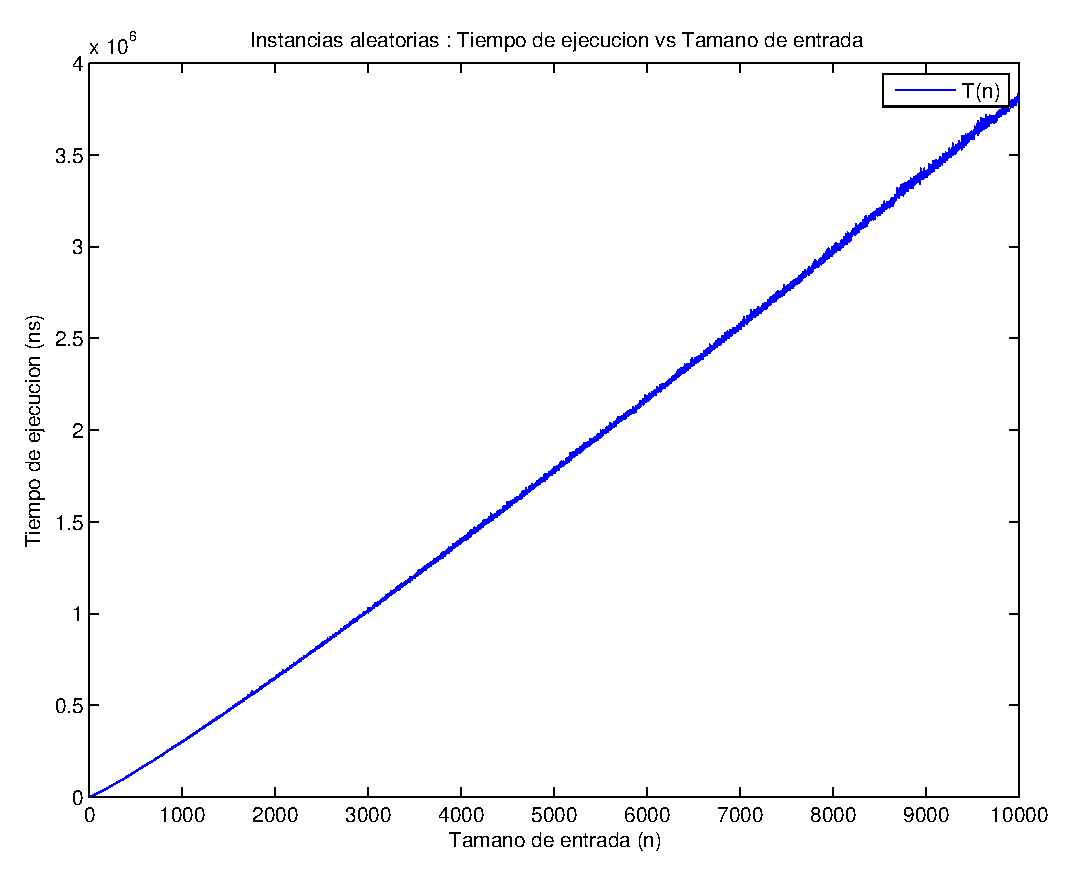
\includegraphics[width=0.5\linewidth]{problema2/graficos/problema2_aleatoria_10000.eps}
    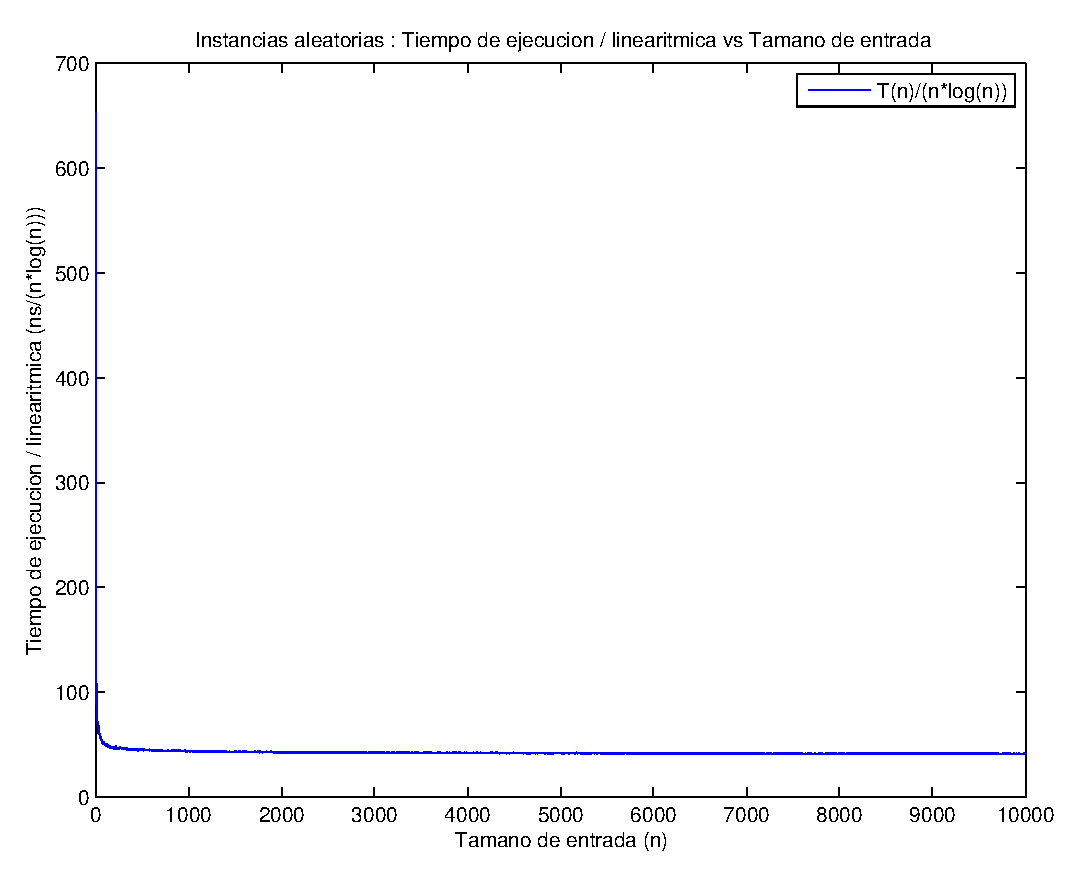
\includegraphics[width=0.5\linewidth]{problema2/graficos/problema2_aleatoria_10000_div_nlogn.eps}
    \caption{Instancias aleatorias, $1 \leq n \leq 10000$. Izquierda: $T(n)$ vs $n$. Derecha: $T(n) / (n * log(n))$ vs $n$.}
    \label{fig:problema2-aleatoria-10000}
  \end{figure}
\end{center}

Además de presentar los datos según fueron medidos, incluímos un gráfico donde se muestra el comportamiento del costo temporal para instancias de tamaño $n$ dividido $n * log(n)$. Esto permite visualizar la tendencia asintótica del cociente $T(n) / (n * log(n))$, que en este caso se aproxima a una constante cercana al valor $50$, sugiriendo dentro del marco de mediciones que $T(n)$ tiende a un crecimiento del orden de $n * log(n)$ para instancias promedio. Esto coincide con el comportamiento observado durante la experimentación del problema \emph{Camiones Sospechosos}, lo cual es de esperarse dado que en ambos casos se utilizó la misma función de ordenamiento para la implementación (ver apéndices \ref{problema1-codigo} y \ref{problema2-codigo}).

Nuevamente, para corroborar que el ciclo posterior al ordenamiento incurre efectivamente en un costo a lo sumo lineal, continuamos la experimentación sobre instancias donde la lista de entrada se encuentra ordenada, eliminando la primer etapa. En este caso, dado que el ciclo no contiene ejecución condicional (siempre ejecuta exactamente la misma cantidad de instrucciones independientemente de la entrada), solo realizamos mediciones sobre instancias pseudo-aleatorias ordenadas según el coeficiente mencionado en \ref{problema2-desarrollo}. En la figura (\ref{fig:problema2-ciclo}) se muestran los resultados.

\begin{center}
  \begin{figure}[H]
    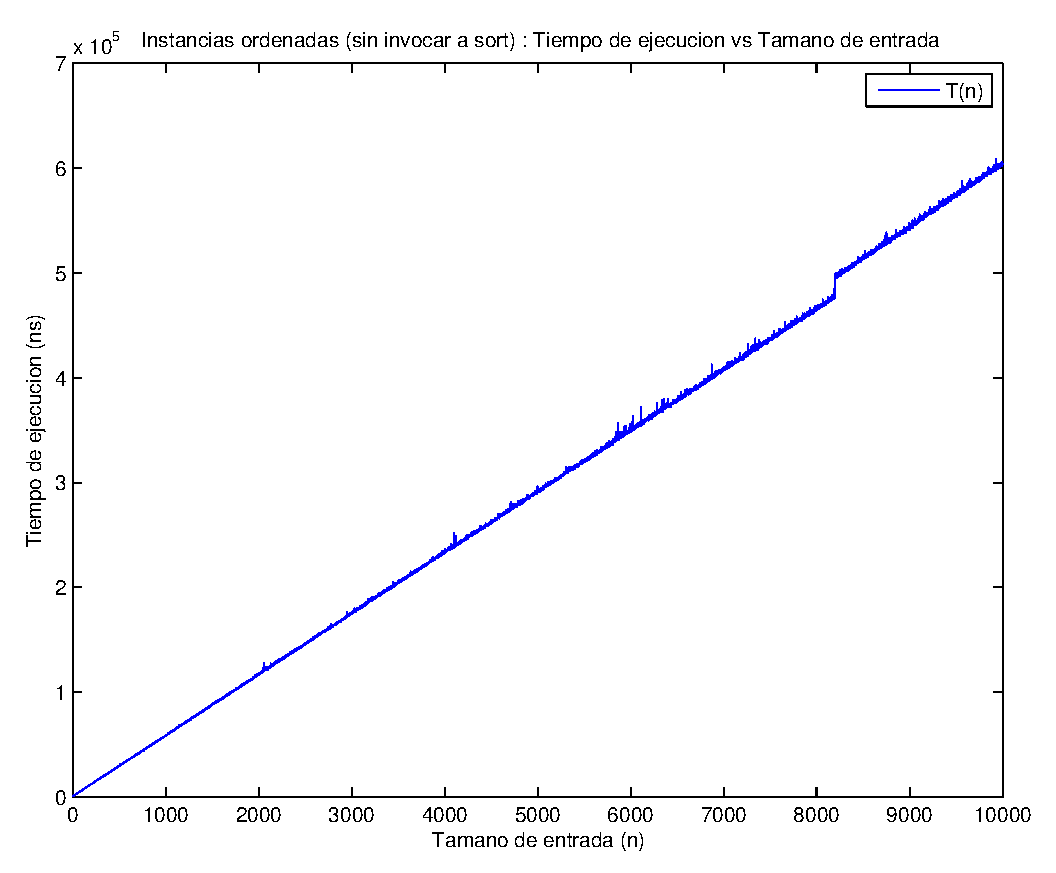
\includegraphics[width=0.5\linewidth]{problema2/graficos/problema2_ordenada_10000.eps}
    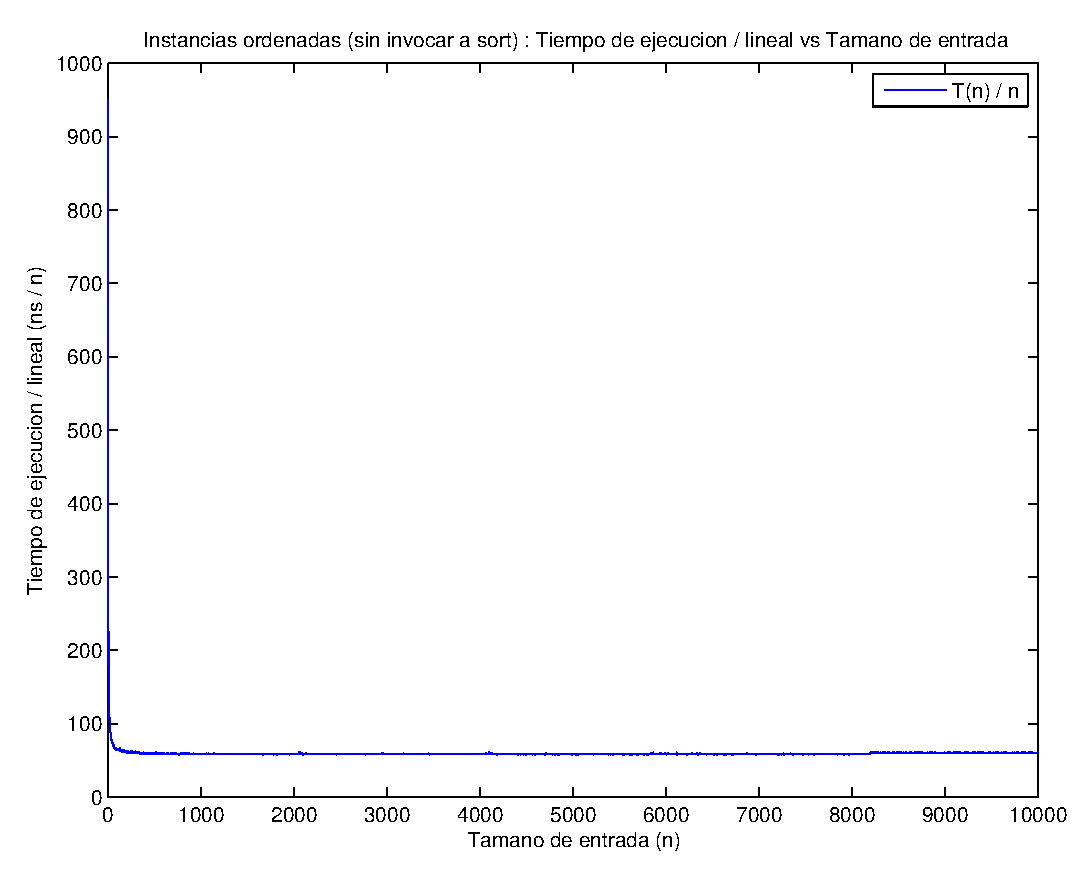
\includegraphics[width=0.5\linewidth]{problema2/graficos/problema2_ordenada_10000_div_n.eps}
  \caption{Instancias aleatorias. $1 \leq n \leq 10000$.}
  \label{fig:problema2-ciclo}
  \end{figure}
\end{center}

Observamos en la curva de costo temporal un crecimiento de orden lineal, con una marcada discontinuidad para $n$ cercano a $8000$. A la vez, incluímos un gráfico mostrando la curva $T(n) / n$ vs $n$\footnote{$T(n)$ en este caso hace referencia a el costo sin la etapa de ordenamiento.}, reiterando sobre la misma técnica utilizada en la sección \ref{problema1-experimentacion}, observando una tendencia hacia un valor constante de aproximadamente $80$ para magnitudes crecientes de $n$. En base a ambas visualizaciones, deducimos que la etapa post-ordenamiento es efectivamente $O(n)$, dado que para la misma no existe distincción entre mejor y peor caso, o caso promedio. Como además es necesario evaluar cada elemento por lo menos una vez al calcular las pérdidas, la etapa es en particular $\Theta(n)$.

Si bien la discontinuidad encontrada no se condice con un comportamiento lineal, aducimos que la misma se debe a cuestiones concretas del contexto de experimentación; por ejemplo, posiblemente debido al tamaño de la memoria caché dado que la posición de la discontinuidad varía cuando realizamos mediciones en equipos de diferentes características.

%Por otro lado, como utilizamos el \emph{sort} de la \emph{stl}, no podemos asegurar si un caso en particular va a ser un ``mejor caso'', o un ``peor caso''. Esto se debe a que, como explicamos anteriormente, el sorting utiliza un \emph{IntroSort} que usa primordialmente un algoritmo similar a \emph{QuickSort}. Por esto al depender del azar, no se puede saber \emph{a priori} si un caso va a ser un ``mejor caso'', o un ``peor caso''.

%Por estas razones, para el ejercicio 2 no incluimos gráficos extra en los cuales hablamos de ``peor caso'' y ``mejor caso''..

\subsection{Resultados y conclusiones}
Dado que el cómputo de la pérdida total tiene un costo fijo determindo por la cantidad de piezas, la variación en el tiempo de ejecución depende exclusivamente del costo de ordenamiento. Por lo tanto, no nos es posible determinar \emph{a priori} si un caso va a resultar mejor o peor para nuestra implementación, sin realizar un complejo análisis de peor caso sobre la función de ordenamiento.

A su vez, la predominancia de la etapa de ordenamiento implica que no va a ser posible mejorar la cota de complejidad teórica de nuestra solución, debido a que los algoritmos de ordenamiento por comparaciones son $\Omega(n * log(n))$.

\newpage


%%%%%%%%%%%%%%%%%%%%%%%%%%%%%%%%%%%%%%%%%%%%%%%%%%%%%%%%%%%%%%%%%%%%%%%%%%%%%%%
%% Problema 2: La joya del Río de la Plata                                   %%
%%%%%%%%%%%%%%%%%%%%%%%%%%%%%%%%%%%%%%%%%%%%%%%%%%%%%%%%%%%%%%%%%%%%%%%%%%%%%%%

\section{Problema 2: La joya del Río de la Plata}

\subsection{Descripción del problema}
Este problema trata sobre un joyero que debe fabricar un conjunto de $n$ piezas cuya materia prima se encuentra en un proceso de depreciación. Para cada pieza \emph{i} de este conjunto, se conoce la cantidad de días que el joyero requiere para su fabricación (\emph{$t_i$}), además de la pérdida diaria (\emph{$p_i$}) que le genera el tener en su posesión la materia prima necesaria para dicha pieza. En función de estos valores, podemos calcular la pérdida total que sufre el joyero durante la fabricación de todas las piezas del conjunto, mediante la siguiente expresión:

$$C(R) = \sum_{i=1}^{n} (t_{R[i]} \sum_{j=i}^{n}p_{R[j]})$$

donde $R[i]$ representa el orden en el cual fue fabricada la $i$-ésima pieza, y $C$ representa el costo o la pérdida total de elegir tal ordenamiento.

Se desea desarrollar un algoritmo que determine un orden óptimo para la fabricación de estas piezas, en el sentido de que minimiza la pérdida total del joyero, y que además compute cuál es dicha pérdida. Como requerimiento adicional, la complejidad del algoritmo utilizado debe ser $O(n^2)$.

A continuación, damos una instancia del problema planteado junto con su solución. Supongamos que tenemos las siguientes piezas:

\begin{center}
  \begin{tabular}{|c|c|c|}
   \hline
   \textbf{Pieza} & \textbf{Pérdida} & \textbf{Tiempo} \\
   \hline
   1 & 3 & 1 \\
   
   2 & 2 & 1 \\
   
   3 & 1 & 1 \\
   \hline
  \end{tabular}
\end{center}

En este ejemplo la solución es la siguiente secuencia:

\textbf{Solución} = [Pieza 1, Pieza 2, Pieza 3]

La pérdida total para esta solución es: $3*1 + 2*2 + 1*3 = 10$

En cambio si eligiéramos como solución otra secuencia, como por ejemplo [Pieza 2, Pieza 1, Pieza 3], la pérdida total sería de: $2*1 + 3*2 + 1*3 = 11$. Si eligiéramos [Pieza 3, Pieza 2, Pieza 1], la pérdida total sería de: $1*1 + 2*2 + 3*3 = 14$.

\subsection{Desarrollo de la solución}
El algoritmo desarrollado para resolver el problema considera como posibles candidatos para fecha de inicio únicamente a los valores del conjunto $\{d_1\;d_2\;...\;d_n\}$, haciendo uso de la siguiente propiedad (demostración en la sección \ref{problema1-demostracion}):

\begin{propiedad}\label{propiedad-candidatos}
Siempre existe un intervalo óptimo $[d, d + D)$ (en el sentido de que comprende la mayor cantidad posible de elementos de la lista) cuyo límite inferior es $d \in \{d_1,d_2,...,d_n\}$.
\end{propiedad}

Para cada candidato $d_i$, se computa la cantidad de elementos contenidos en el intervalo $[d_i, d_i + D)$, guardando un registro del día $d$ para el cual dicha cantidad es mayor. Finalmente, se emite como solución el valor de $d$ y la cantidad $c$ de números contenidos en su respectivo intervalo.

Dado el requerimiento de que la solución tenga complejidad temporal subcuadrática, no es viable el procedimiento ingenuo de tomar cada día de la lista $d_i$ y, para cada valor $1 \leq j \leq n$, evaluar la condición de pertenencia $d_i \leq d_j < d_i + D$.

En cambio, la resolución propuesta realiza primeramente un ordenamiento sobre la lista, y luego recorre la misma linealmente mediante dos índices $i,j$, manteniendo en cada iteración el siguiente invariante\footnote{Los subíndices refieren a los elementos de la lista ya ordenada}:

$$(\forall k: i \leq k < j)\;d_k \in [d_i, d_i + D)$$

Si sucede que $d_{i-1} = d_i$, se está en presencia de un candidato que ya ha sido contemplado, y por lo tanto se saltea. De lo contrario, vale $d_{i-1} < d_i$ y por lo tanto $d_i$ es el primer elemento de la lista contenido en $[d_i, d_i + D)$. Esto permite computar la cantidad total de elementos contenidos en el intervalo mediante la expresión $j - i$, cuyo valor se utiliza para actualizar la solución parcial.

Adicionalmente, la búsqueda del máximo $j$ que cumple el invariante puede realizarse a partir del valor de $j$ de la iteración anterior\footnote{En el caso base, se toma $j = 1$ para comenzar a partir del primer elemento.}, fundamentado en la siguiente propiedad (demostración en la sección \ref{problema1-demostracion}):

\begin{propiedad}\label{propiedad-maximo-j}
$$((\forall k: i \leq k < j)\;d_k \in [d_i, d_i + D)) \Rightarrow ((\forall k: i + 1 \leq k < j)\;d_k \in [d_{i+1}, d_{i+1} + D))$$
\end{propiedad}

Es decir, si vale el invariante para $(i,j)$, entonces vale para $(i+1,j)$. Esto permite obtener el valor máximo de $j$ correspondiente a cada $i$ mediante un único recorrido lineal, ya que $j$ nunca decrece. En la figura \ref{problema1-pseudo} se incluye pseudocódigo describiendo el algoritmo desarrollado en detalle, y en el apéndice \ref{problema1-codigo} se incluye el código completo.

\begin{center}
\begin{figure}[H]
    \begin{pseudo}
        \Procedure{Camiones-Sospechosos}{$D, n, \langle d_1, \ldots, d_n \rangle$}
            \State $ordenar(\langle d_1, \ldots, d_n \rangle)$ \Ode{n\;log(n)}
            \State $d \leftarrow 0, c \leftarrow 0$ \Ode{1}
            \State $i \leftarrow 1$, $j \leftarrow 1$ \Ode{1}
            \While{$i \leq n$} \Ode{1}
                \If{$0 < i \land d_{i-1} = d_i$}
                    \textbf{continue} \Ode{1}
                \EndIf
                \While{$(j \leq n) \land (d_i \leq d_j < d_i + D)$} \Ode{1}
                    \State $j \leftarrow j + 1$ \Ode{1}
                \EndWhile
                \If{$c < j - i$} \Ode{1}
                    \State $c \leftarrow j - i$ \Ode{1}
                    \State $d \leftarrow i$ \Ode{1}
                \EndIf
                \State $i \leftarrow i + 1$ \Ode{1}
            \EndWhile
            \Return $d$, $c$
        \EndProcedure
    \end{pseudo}
    \caption{Camiones Sospechosos. Pseudocódigo.}
    \label{problema1-pseudo}
\end{figure}
\end{center}


\subsection{Demostración de correctitud}
Para demostrar la correctitud del algoritmo propuesto, es necesario probar esencialmente dos afirmaciones mencionadas en la sección \ref{problema1-desarrollo}. En primer lugar, debe justificarse que entre los intervalos empezados en los $d_i$ siempre va a existir un máximo o, formalmente, se debe demostrar la Propiedad \ref{propiedad-candidatos}. Luego, es importante argumentar por qué el ciclo del algoritmo computa efectivamente la cantidad de elementos de la lista contenidos en el intervalo asociado a cada candidato.

\subsubsection{Demostración de la Propiedad \ref{propiedad-candidatos}}

Dada una instancia $<D,\;n,\;l = [d_1, d_2, ..., d_n]>$, se quiere probar que siempre existe un intervalo óptimo $[d, d + D)$ (en el sentido de que comprende la mayor cantidad posible de elementos de la lista $l$) cuyo límite inferior es $d \in \{d_1,d_2,...,d_n\}$.

Como cualquier valor $d$ natural genera un intervalo $[d, d + D)$ válido, el conjunto de posibles soluciones es no vacío. Como además cualquier solución posible contiene entre 0 y $n$ elementos de la lista, necesariamente existe solución óptima. Sea $d'$ tal que $[d', d' + D)$ es un intervalo óptimo.

\begin{itemize}
  \item Si $(\nexists\;i : 1 \leq i \leq n)\;d' \leq d_i$, entonces el intervalo $[d', d' + D)$ no contiene ningún elemento de la lista. Esto es absurdo porque cualquier intervalo $[d_i, d_i + D)$ contiene al menos un elemento, y sería mejor que el óptimo.
  \item De lo contrario, se puede definir $d^*$ como el menor elemento de la lista que es mayor o igual a $d'$; es decir: $d^* = min\;\{\;d_i : 1 \leq i \leq n \land d' \leq d_i\;\}$.

  Luego, $\forall\;i : 1 \leq i \leq n$:
  
  \begin{itemize}
    \item Como $d^*$ es el menor elemento que cumple la propiedad de ser mayor o igual que $d'$:
    $$d' \leq d_i \rightarrow d^*\leq d_i$$
    \item Como $d' \leq d^*$ por definición, se desprende que $d' + D \leq d^* + D$, y por lo tanto:
    $$(d_i < d' + D) \rightarrow (d_i < d^* + D)$$
  \end{itemize}
  Entonces, vale que todo elemento contenido en el intervalo óptimo también está contenido en el intervalo $[d^*, d^* + D)$. Como $d^* \in \{d_1,d_2,...,d_n\}$, queda demostrada la propiedad.
\end{itemize}

\subsubsection{Correctitud del ciclo}

En la inicialización previa al ciclo, se configura $(i, j) \leftarrow (1, 1)$ y por lo tanto, vale trivialmente el invariante:

$$(\forall k: i \leq k < j)\;d_k \in [d_i, d_i + D)$$

El cuerpo del ciclo se ejecuta únicamente para el primer elemento de la lista, y para todos aquellos que no sean iguales al inmediatamente anterior. Como la lista está ordenada, esto es equivalente a evaluar únicamente la primera aparición de cada valor dentro de la lista, ignorando sus posibles repeticiones posteriores.

El ciclo interno tiene la única función de incrementar el valor de $j$. La guarda del mismo es:

$$(j \leq n) \land (d_i \leq d_j < d_i + D) \equiv (j \leq n) \land d_j \in [d_i, d_i + D)$$

Es decir, $j$ jamás se incrementa si el $j$-ésimo elemento no pertenece al intervalo $[d_i, d_i + D)$. Esto mantiene el invariante, evitando que algún elemento con índice menor a $j$ no pertenezca al intervalo del candidato en evaluación. Como además $j$ se incrementa tantas veces como sea posible sin romper el invariante, esto garantiza que al terminar el ciclo interno la variable tendrá su valor máximo (cuando $j = n + 1$ ó $d_j \notin [d_i, d_i + D)$).

Luego, $d_i$ es el primer elemento de la lista contenido en $[d_i, d_i + D)$ por no tener predecesor o por ser mayor que el mismo. Además, $d_{j-1}$ es el último elemento de la lista contenido en $[d_i, d_i + D)$ por no tener sucesor, o porque lo garantiza el invariante en caso contrario. De ello se desprende que existen $(j - 1) - i + 1 = j - i$ elementos de la lista contenidos en el intervalo, por lo cual es el valor que se utiliza para actualizar el estado de la solución parcial.

Por último, es necesario probar que el invariante se mantiene al incrementar $i$ al final del ciclo. Esto es equivalente a demostrar la propiedad \ref{propiedad-maximo-j}.

\subsubsection{Demostración de la Propiedad \ref{propiedad-maximo-j}}

Si el invariante de ciclo es válido para el par $(i,j)$, entonces también lo es para $(i + 1,j)$. Formalmente:

$$((\forall k: i \leq k < j)\;d_k \in [d_i, d_i + D)) \Rightarrow ((\forall k: i + 1 \leq k < j)\;d_k \in [d_{i+1}, d_{i+1} + D))$$

De la verdad del antecedente, y dado que los elementos $d_i$ están ordenados al comenzar el ciclo, se deducen las siguientes propiedades para todo $k'$ tal que $i + 1 \leq k'< j$:

\begin{enumerate}
  \item $d_{i+1} \leq d_{k'}$               \hfill        por estar ordenados, ya que $i+1 \leq k'$
  \item $d_i \leq d_{i+1}$                  \hfill        por estar ordenados
  \item $d_{i} + D \leq d_{i + 1} +D$       \hfill        se deduce de 2
  \item $d_{k'} < d_i +D$                   \hfill        por el antecedente, ya que $d_{k'} \in [d_i,d_i +D)$
  \item $d_{k'} < d_{i+1} +D$               \hfill        se deduce de 3 y 4
\end{enumerate}

En base a 1 y 5, vale que $d_{k'} \in [d_{i+1}, d_{i+1} + D)$, y queda demostrada la propiedad.

\subsection{Complejidad temporal}
El pseudocódigo de la solución (Figura \ref{problema1-pseudo}) incluye al final de cada línea la complejidad temporal de las instrucciones contenidas en la misma.

En primer lugar, la etapa de ordenamiento es realizable en tiempo $O(n\;log\;n)$ mediante conocidos algoritmos como \emph{Mergesort}, \emph{Heapsort} o \emph{Introsort}.

Luego, dado que $j$ se inicializa en $1$ y su valor es incrementado en el cuerpo del ciclo interno, la guarda del mismo no puede ser verdadera más de $n$ veces. Como además siempre vale que $d_i \leq d_i < d_i + D$, este se ejecuta al menos una vez por cada valor de $i$. Por lo tanto, la operación $j \leftarrow j + 1$ se ejecuta $n$ veces, incurriendo en un costo lineal en $n$ en la totalidad del algoritmo, y no se ejecuta $n$ veces por cada valor de $i$.

Por otro lado, el ciclo externo se ejecuta exactamente $n$ veces, con $i = 1, ..., n$. En peor caso, los elementos son todos distintos y jamás se saltea el cuerpo del ciclo. Las operaciones de actualización del máximo tienen un costo constante (incluso si hay que realizar la actualización), por lo cual en la totalidad del algoritmo comprenden una cantidad de operaciones proporcional a $n$.

Buscar el máximo tiene una complejidad $O(n)$. Por esto, la etapa de ordenamiento (la cual tiene una complejidad de $O(n*log(n))$) domina la complejidad del algoritmo, permitiendo dar la cota $O(n*log(n))$ para la solución.

\subsection{Experimentación}
% Para experimentar, utilizamos una computadora con las siguientes características:

% \begin{itemize}
%  \item Procesador: 
%  \item RAM: 
% \end{itemize}

Al igual que en el problema \emph{Camiones Sospechosos}, la solución propuesta tiene la característica de que la complejidad temporal del algoritmo es dominada por la etapa de ordenamiento. Por esta razón, lo que mencionamos en la sección \ref{problema1-experimentacion} también vale en este caso: las instancias utilizadas para la medición se generaron de forma pseudo-aleatoria, limitando el análisis de los resultados al rendimiento de caso promedio.

Medimos el tiempo de ejecución al resolver instancias de entre 1 y 10000 piezas, según las consideraciones de la sección \ref{consideraciones-mediciones}, permitiendo graficar el costo temporal de la implementación en función del tamaño de entrada $T(n)$. En la figura (\ref{fig:problema2-aleatoria-10000}) se observan los resultados obtenidos.

\begin{center}
  \begin{figure}[H]
    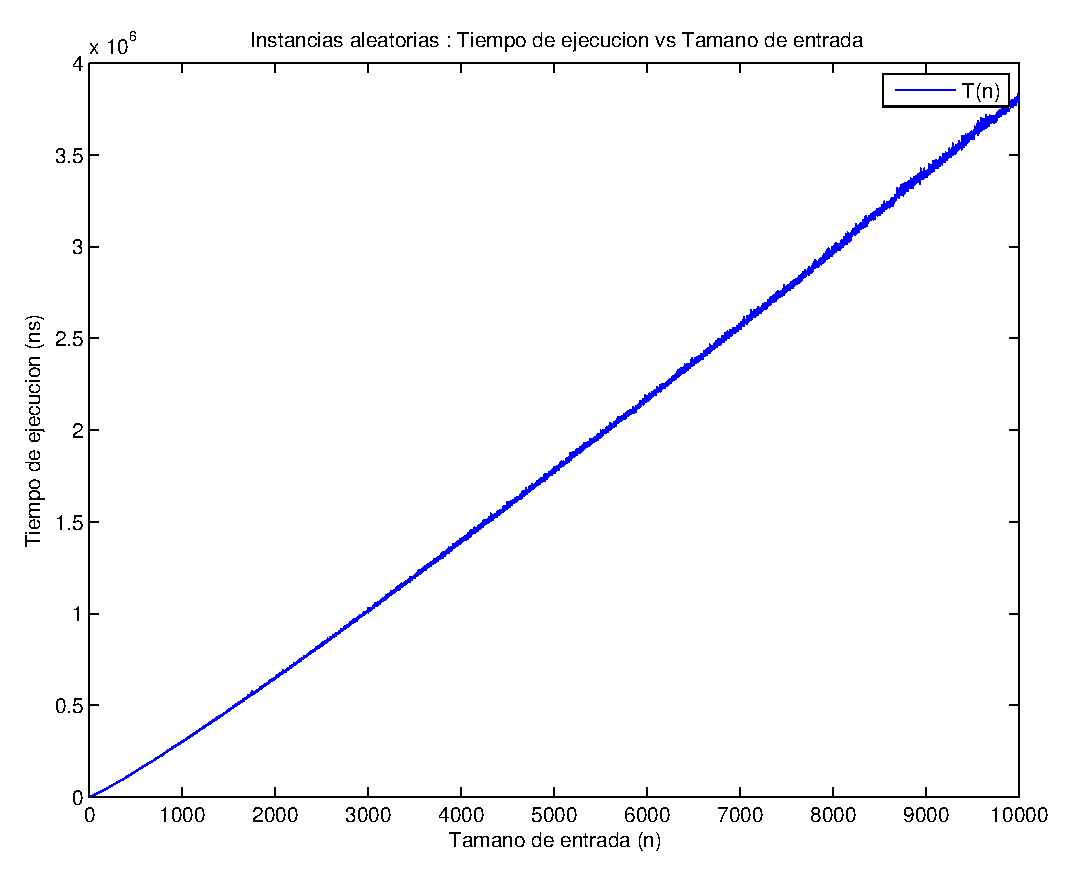
\includegraphics[width=0.5\linewidth]{problema2/graficos/problema2_aleatoria_10000.eps}
    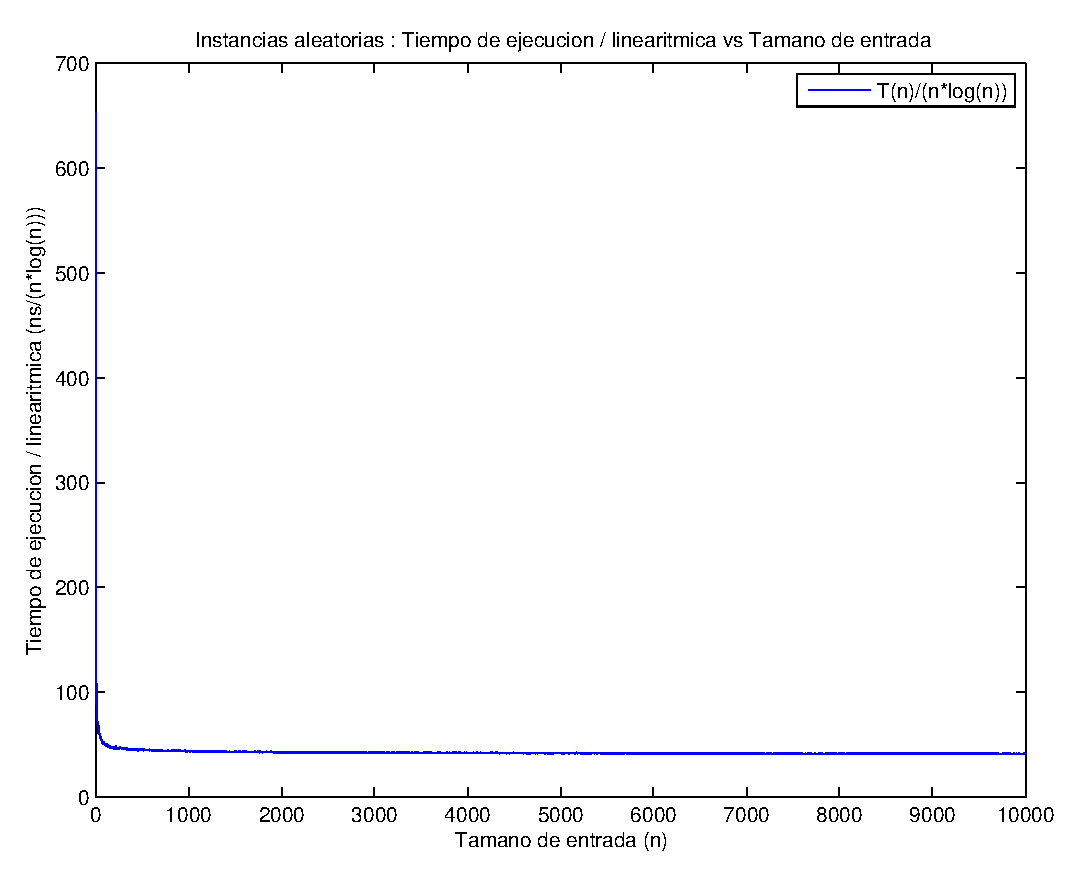
\includegraphics[width=0.5\linewidth]{problema2/graficos/problema2_aleatoria_10000_div_nlogn.eps}
    \caption{Instancias aleatorias, $1 \leq n \leq 10000$. Izquierda: $T(n)$ vs $n$. Derecha: $T(n) / (n * log(n))$ vs $n$.}
    \label{fig:problema2-aleatoria-10000}
  \end{figure}
\end{center}

Además de presentar los datos según fueron medidos, incluímos un gráfico donde se muestra el comportamiento del costo temporal para instancias de tamaño $n$ dividido $n * log(n)$. Esto permite visualizar la tendencia asintótica del cociente $T(n) / (n * log(n))$, que en este caso se aproxima a una constante cercana al valor $50$, sugiriendo dentro del marco de mediciones que $T(n)$ tiende a un crecimiento del orden de $n * log(n)$ para instancias promedio. Esto coincide con el comportamiento observado durante la experimentación del problema \emph{Camiones Sospechosos}, lo cual es de esperarse dado que en ambos casos se utilizó la misma función de ordenamiento para la implementación (ver apéndices \ref{problema1-codigo} y \ref{problema2-codigo}).

Nuevamente, para corroborar que el ciclo posterior al ordenamiento incurre efectivamente en un costo a lo sumo lineal, continuamos la experimentación sobre instancias donde la lista de entrada se encuentra ordenada, eliminando la primer etapa. En este caso, dado que el ciclo no contiene ejecución condicional (siempre ejecuta exactamente la misma cantidad de instrucciones independientemente de la entrada), solo realizamos mediciones sobre instancias pseudo-aleatorias ordenadas según el coeficiente mencionado en \ref{problema2-desarrollo}. En la figura (\ref{fig:problema2-ciclo}) se muestran los resultados.

\begin{center}
  \begin{figure}[H]
    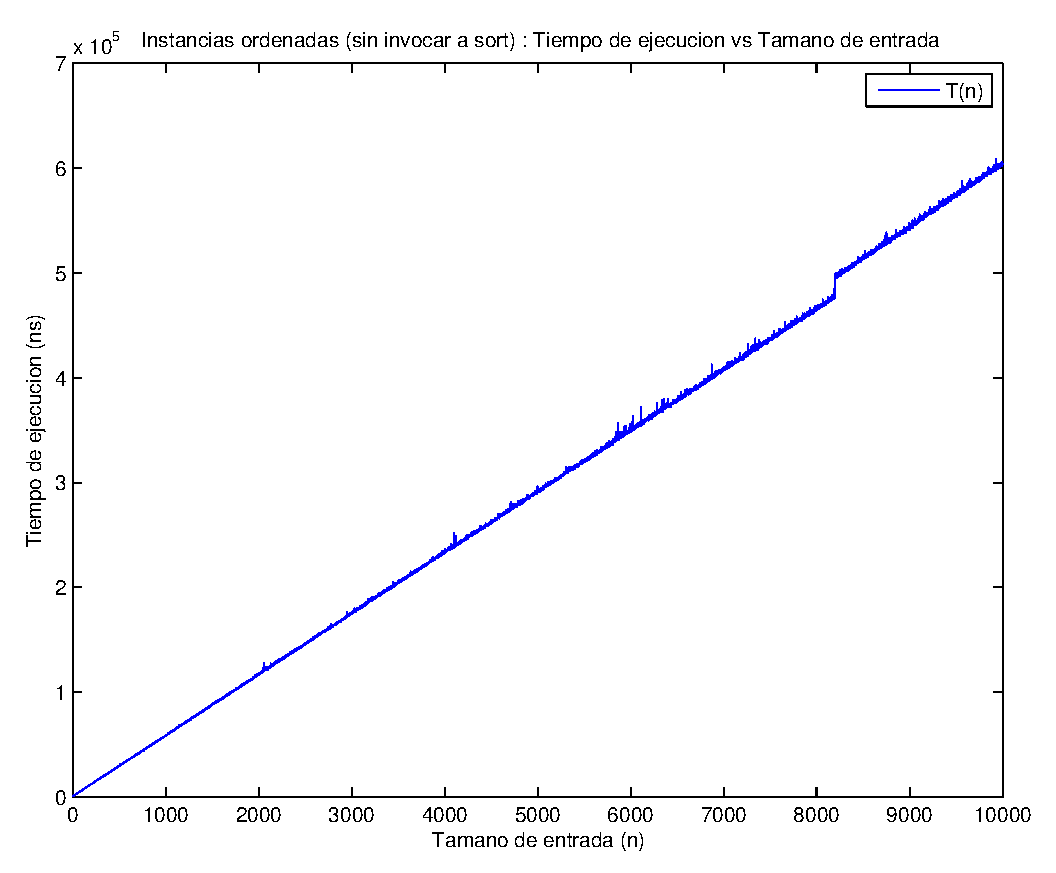
\includegraphics[width=0.5\linewidth]{problema2/graficos/problema2_ordenada_10000.eps}
    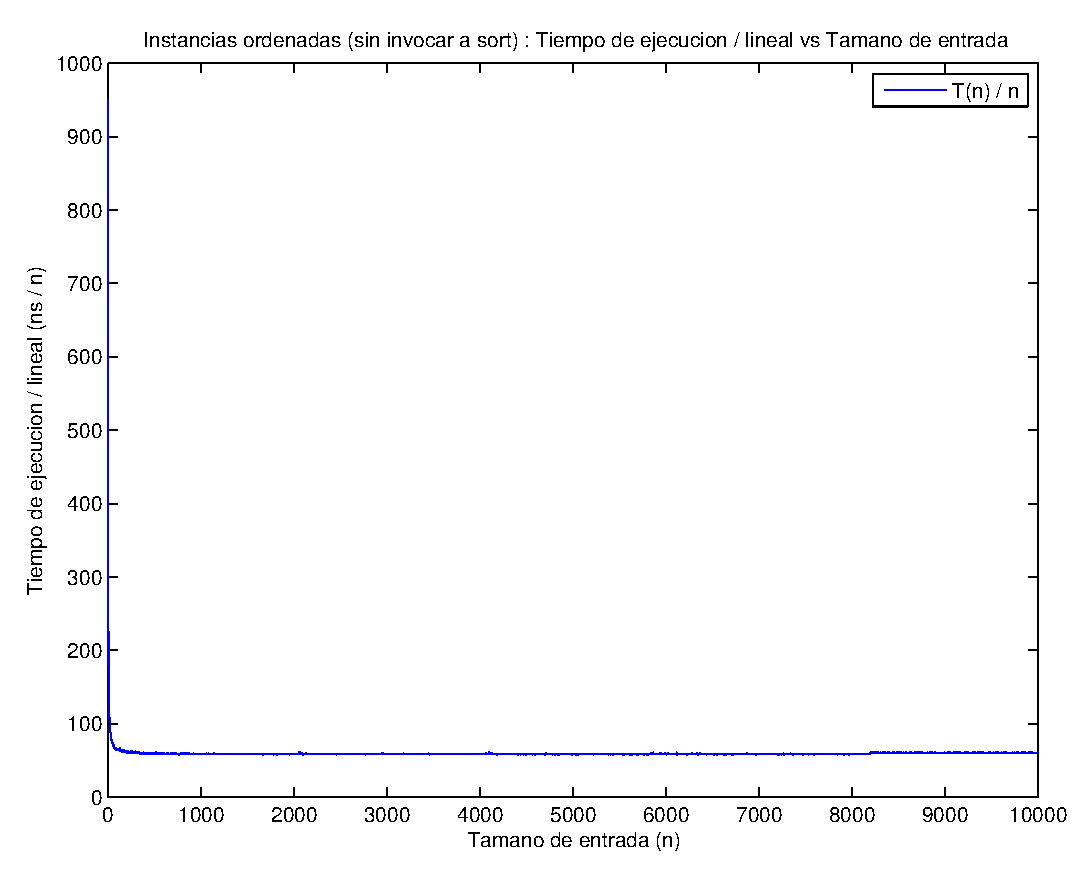
\includegraphics[width=0.5\linewidth]{problema2/graficos/problema2_ordenada_10000_div_n.eps}
  \caption{Instancias aleatorias. $1 \leq n \leq 10000$.}
  \label{fig:problema2-ciclo}
  \end{figure}
\end{center}

Observamos en la curva de costo temporal un crecimiento de orden lineal, con una marcada discontinuidad para $n$ cercano a $8000$. A la vez, incluímos un gráfico mostrando la curva $T(n) / n$ vs $n$\footnote{$T(n)$ en este caso hace referencia a el costo sin la etapa de ordenamiento.}, reiterando sobre la misma técnica utilizada en la sección \ref{problema1-experimentacion}, observando una tendencia hacia un valor constante de aproximadamente $80$ para magnitudes crecientes de $n$. En base a ambas visualizaciones, deducimos que la etapa post-ordenamiento es efectivamente $O(n)$, dado que para la misma no existe distincción entre mejor y peor caso, o caso promedio. Como además es necesario evaluar cada elemento por lo menos una vez al calcular las pérdidas, la etapa es en particular $\Theta(n)$.

Si bien la discontinuidad encontrada no se condice con un comportamiento lineal, aducimos que la misma se debe a cuestiones concretas del contexto de experimentación; por ejemplo, posiblemente debido al tamaño de la memoria caché dado que la posición de la discontinuidad varía cuando realizamos mediciones en equipos de diferentes características.

%Por otro lado, como utilizamos el \emph{sort} de la \emph{stl}, no podemos asegurar si un caso en particular va a ser un ``mejor caso'', o un ``peor caso''. Esto se debe a que, como explicamos anteriormente, el sorting utiliza un \emph{IntroSort} que usa primordialmente un algoritmo similar a \emph{QuickSort}. Por esto al depender del azar, no se puede saber \emph{a priori} si un caso va a ser un ``mejor caso'', o un ``peor caso''.

%Por estas razones, para el ejercicio 2 no incluimos gráficos extra en los cuales hablamos de ``peor caso'' y ``mejor caso''..

\subsection{Resultados y conclusiones}
Dado que el cómputo de la pérdida total tiene un costo fijo determindo por la cantidad de piezas, la variación en el tiempo de ejecución depende exclusivamente del costo de ordenamiento. Por lo tanto, no nos es posible determinar \emph{a priori} si un caso va a resultar mejor o peor para nuestra implementación, sin realizar un complejo análisis de peor caso sobre la función de ordenamiento.

A su vez, la predominancia de la etapa de ordenamiento implica que no va a ser posible mejorar la cota de complejidad teórica de nuestra solución, debido a que los algoritmos de ordenamiento por comparaciones son $\Omega(n * log(n))$.

\newpage


%%%%%%%%%%%%%%%%%%%%%%%%%%%%%%%%%%%%%%%%%%%%%%%%%%%%%%%%%%%%%%%%%%%%%%%%%%%%%%%
%% Problema 3: Rompecolores                                                  %%
%%%%%%%%%%%%%%%%%%%%%%%%%%%%%%%%%%%%%%%%%%%%%%%%%%%%%%%%%%%%%%%%%%%%%%%%%%%%%%%

\section{Problema 3: Rompecolores}

\subsection{Descripción del problema}
Este problema trata sobre un joyero que debe fabricar un conjunto de $n$ piezas cuya materia prima se encuentra en un proceso de depreciación. Para cada pieza \emph{i} de este conjunto, se conoce la cantidad de días que el joyero requiere para su fabricación (\emph{$t_i$}), además de la pérdida diaria (\emph{$p_i$}) que le genera el tener en su posesión la materia prima necesaria para dicha pieza. En función de estos valores, podemos calcular la pérdida total que sufre el joyero durante la fabricación de todas las piezas del conjunto, mediante la siguiente expresión:

$$C(R) = \sum_{i=1}^{n} (t_{R[i]} \sum_{j=i}^{n}p_{R[j]})$$

donde $R[i]$ representa el orden en el cual fue fabricada la $i$-ésima pieza, y $C$ representa el costo o la pérdida total de elegir tal ordenamiento.

Se desea desarrollar un algoritmo que determine un orden óptimo para la fabricación de estas piezas, en el sentido de que minimiza la pérdida total del joyero, y que además compute cuál es dicha pérdida. Como requerimiento adicional, la complejidad del algoritmo utilizado debe ser $O(n^2)$.

A continuación, damos una instancia del problema planteado junto con su solución. Supongamos que tenemos las siguientes piezas:

\begin{center}
  \begin{tabular}{|c|c|c|}
   \hline
   \textbf{Pieza} & \textbf{Pérdida} & \textbf{Tiempo} \\
   \hline
   1 & 3 & 1 \\
   
   2 & 2 & 1 \\
   
   3 & 1 & 1 \\
   \hline
  \end{tabular}
\end{center}

En este ejemplo la solución es la siguiente secuencia:

\textbf{Solución} = [Pieza 1, Pieza 2, Pieza 3]

La pérdida total para esta solución es: $3*1 + 2*2 + 1*3 = 10$

En cambio si eligiéramos como solución otra secuencia, como por ejemplo [Pieza 2, Pieza 1, Pieza 3], la pérdida total sería de: $2*1 + 3*2 + 1*3 = 11$. Si eligiéramos [Pieza 3, Pieza 2, Pieza 1], la pérdida total sería de: $1*1 + 2*2 + 3*3 = 14$.

\subsection{Desarrollo de la solución}
El algoritmo desarrollado para resolver el problema considera como posibles candidatos para fecha de inicio únicamente a los valores del conjunto $\{d_1\;d_2\;...\;d_n\}$, haciendo uso de la siguiente propiedad (demostración en la sección \ref{problema1-demostracion}):

\begin{propiedad}\label{propiedad-candidatos}
Siempre existe un intervalo óptimo $[d, d + D)$ (en el sentido de que comprende la mayor cantidad posible de elementos de la lista) cuyo límite inferior es $d \in \{d_1,d_2,...,d_n\}$.
\end{propiedad}

Para cada candidato $d_i$, se computa la cantidad de elementos contenidos en el intervalo $[d_i, d_i + D)$, guardando un registro del día $d$ para el cual dicha cantidad es mayor. Finalmente, se emite como solución el valor de $d$ y la cantidad $c$ de números contenidos en su respectivo intervalo.

Dado el requerimiento de que la solución tenga complejidad temporal subcuadrática, no es viable el procedimiento ingenuo de tomar cada día de la lista $d_i$ y, para cada valor $1 \leq j \leq n$, evaluar la condición de pertenencia $d_i \leq d_j < d_i + D$.

En cambio, la resolución propuesta realiza primeramente un ordenamiento sobre la lista, y luego recorre la misma linealmente mediante dos índices $i,j$, manteniendo en cada iteración el siguiente invariante\footnote{Los subíndices refieren a los elementos de la lista ya ordenada}:

$$(\forall k: i \leq k < j)\;d_k \in [d_i, d_i + D)$$

Si sucede que $d_{i-1} = d_i$, se está en presencia de un candidato que ya ha sido contemplado, y por lo tanto se saltea. De lo contrario, vale $d_{i-1} < d_i$ y por lo tanto $d_i$ es el primer elemento de la lista contenido en $[d_i, d_i + D)$. Esto permite computar la cantidad total de elementos contenidos en el intervalo mediante la expresión $j - i$, cuyo valor se utiliza para actualizar la solución parcial.

Adicionalmente, la búsqueda del máximo $j$ que cumple el invariante puede realizarse a partir del valor de $j$ de la iteración anterior\footnote{En el caso base, se toma $j = 1$ para comenzar a partir del primer elemento.}, fundamentado en la siguiente propiedad (demostración en la sección \ref{problema1-demostracion}):

\begin{propiedad}\label{propiedad-maximo-j}
$$((\forall k: i \leq k < j)\;d_k \in [d_i, d_i + D)) \Rightarrow ((\forall k: i + 1 \leq k < j)\;d_k \in [d_{i+1}, d_{i+1} + D))$$
\end{propiedad}

Es decir, si vale el invariante para $(i,j)$, entonces vale para $(i+1,j)$. Esto permite obtener el valor máximo de $j$ correspondiente a cada $i$ mediante un único recorrido lineal, ya que $j$ nunca decrece. En la figura \ref{problema1-pseudo} se incluye pseudocódigo describiendo el algoritmo desarrollado en detalle, y en el apéndice \ref{problema1-codigo} se incluye el código completo.

\begin{center}
\begin{figure}[H]
    \begin{pseudo}
        \Procedure{Camiones-Sospechosos}{$D, n, \langle d_1, \ldots, d_n \rangle$}
            \State $ordenar(\langle d_1, \ldots, d_n \rangle)$ \Ode{n\;log(n)}
            \State $d \leftarrow 0, c \leftarrow 0$ \Ode{1}
            \State $i \leftarrow 1$, $j \leftarrow 1$ \Ode{1}
            \While{$i \leq n$} \Ode{1}
                \If{$0 < i \land d_{i-1} = d_i$}
                    \textbf{continue} \Ode{1}
                \EndIf
                \While{$(j \leq n) \land (d_i \leq d_j < d_i + D)$} \Ode{1}
                    \State $j \leftarrow j + 1$ \Ode{1}
                \EndWhile
                \If{$c < j - i$} \Ode{1}
                    \State $c \leftarrow j - i$ \Ode{1}
                    \State $d \leftarrow i$ \Ode{1}
                \EndIf
                \State $i \leftarrow i + 1$ \Ode{1}
            \EndWhile
            \Return $d$, $c$
        \EndProcedure
    \end{pseudo}
    \caption{Camiones Sospechosos. Pseudocódigo.}
    \label{problema1-pseudo}
\end{figure}
\end{center}


\subsection{Demostración de correctitud}
Para demostrar la correctitud del algoritmo propuesto, es necesario probar esencialmente dos afirmaciones mencionadas en la sección \ref{problema1-desarrollo}. En primer lugar, debe justificarse que entre los intervalos empezados en los $d_i$ siempre va a existir un máximo o, formalmente, se debe demostrar la Propiedad \ref{propiedad-candidatos}. Luego, es importante argumentar por qué el ciclo del algoritmo computa efectivamente la cantidad de elementos de la lista contenidos en el intervalo asociado a cada candidato.

\subsubsection{Demostración de la Propiedad \ref{propiedad-candidatos}}

Dada una instancia $<D,\;n,\;l = [d_1, d_2, ..., d_n]>$, se quiere probar que siempre existe un intervalo óptimo $[d, d + D)$ (en el sentido de que comprende la mayor cantidad posible de elementos de la lista $l$) cuyo límite inferior es $d \in \{d_1,d_2,...,d_n\}$.

Como cualquier valor $d$ natural genera un intervalo $[d, d + D)$ válido, el conjunto de posibles soluciones es no vacío. Como además cualquier solución posible contiene entre 0 y $n$ elementos de la lista, necesariamente existe solución óptima. Sea $d'$ tal que $[d', d' + D)$ es un intervalo óptimo.

\begin{itemize}
  \item Si $(\nexists\;i : 1 \leq i \leq n)\;d' \leq d_i$, entonces el intervalo $[d', d' + D)$ no contiene ningún elemento de la lista. Esto es absurdo porque cualquier intervalo $[d_i, d_i + D)$ contiene al menos un elemento, y sería mejor que el óptimo.
  \item De lo contrario, se puede definir $d^*$ como el menor elemento de la lista que es mayor o igual a $d'$; es decir: $d^* = min\;\{\;d_i : 1 \leq i \leq n \land d' \leq d_i\;\}$.

  Luego, $\forall\;i : 1 \leq i \leq n$:
  
  \begin{itemize}
    \item Como $d^*$ es el menor elemento que cumple la propiedad de ser mayor o igual que $d'$:
    $$d' \leq d_i \rightarrow d^*\leq d_i$$
    \item Como $d' \leq d^*$ por definición, se desprende que $d' + D \leq d^* + D$, y por lo tanto:
    $$(d_i < d' + D) \rightarrow (d_i < d^* + D)$$
  \end{itemize}
  Entonces, vale que todo elemento contenido en el intervalo óptimo también está contenido en el intervalo $[d^*, d^* + D)$. Como $d^* \in \{d_1,d_2,...,d_n\}$, queda demostrada la propiedad.
\end{itemize}

\subsubsection{Correctitud del ciclo}

En la inicialización previa al ciclo, se configura $(i, j) \leftarrow (1, 1)$ y por lo tanto, vale trivialmente el invariante:

$$(\forall k: i \leq k < j)\;d_k \in [d_i, d_i + D)$$

El cuerpo del ciclo se ejecuta únicamente para el primer elemento de la lista, y para todos aquellos que no sean iguales al inmediatamente anterior. Como la lista está ordenada, esto es equivalente a evaluar únicamente la primera aparición de cada valor dentro de la lista, ignorando sus posibles repeticiones posteriores.

El ciclo interno tiene la única función de incrementar el valor de $j$. La guarda del mismo es:

$$(j \leq n) \land (d_i \leq d_j < d_i + D) \equiv (j \leq n) \land d_j \in [d_i, d_i + D)$$

Es decir, $j$ jamás se incrementa si el $j$-ésimo elemento no pertenece al intervalo $[d_i, d_i + D)$. Esto mantiene el invariante, evitando que algún elemento con índice menor a $j$ no pertenezca al intervalo del candidato en evaluación. Como además $j$ se incrementa tantas veces como sea posible sin romper el invariante, esto garantiza que al terminar el ciclo interno la variable tendrá su valor máximo (cuando $j = n + 1$ ó $d_j \notin [d_i, d_i + D)$).

Luego, $d_i$ es el primer elemento de la lista contenido en $[d_i, d_i + D)$ por no tener predecesor o por ser mayor que el mismo. Además, $d_{j-1}$ es el último elemento de la lista contenido en $[d_i, d_i + D)$ por no tener sucesor, o porque lo garantiza el invariante en caso contrario. De ello se desprende que existen $(j - 1) - i + 1 = j - i$ elementos de la lista contenidos en el intervalo, por lo cual es el valor que se utiliza para actualizar el estado de la solución parcial.

Por último, es necesario probar que el invariante se mantiene al incrementar $i$ al final del ciclo. Esto es equivalente a demostrar la propiedad \ref{propiedad-maximo-j}.

\subsubsection{Demostración de la Propiedad \ref{propiedad-maximo-j}}

Si el invariante de ciclo es válido para el par $(i,j)$, entonces también lo es para $(i + 1,j)$. Formalmente:

$$((\forall k: i \leq k < j)\;d_k \in [d_i, d_i + D)) \Rightarrow ((\forall k: i + 1 \leq k < j)\;d_k \in [d_{i+1}, d_{i+1} + D))$$

De la verdad del antecedente, y dado que los elementos $d_i$ están ordenados al comenzar el ciclo, se deducen las siguientes propiedades para todo $k'$ tal que $i + 1 \leq k'< j$:

\begin{enumerate}
  \item $d_{i+1} \leq d_{k'}$               \hfill        por estar ordenados, ya que $i+1 \leq k'$
  \item $d_i \leq d_{i+1}$                  \hfill        por estar ordenados
  \item $d_{i} + D \leq d_{i + 1} +D$       \hfill        se deduce de 2
  \item $d_{k'} < d_i +D$                   \hfill        por el antecedente, ya que $d_{k'} \in [d_i,d_i +D)$
  \item $d_{k'} < d_{i+1} +D$               \hfill        se deduce de 3 y 4
\end{enumerate}

En base a 1 y 5, vale que $d_{k'} \in [d_{i+1}, d_{i+1} + D)$, y queda demostrada la propiedad.

\subsection{Complejidad temporal}
El pseudocódigo de la solución (Figura \ref{problema1-pseudo}) incluye al final de cada línea la complejidad temporal de las instrucciones contenidas en la misma.

En primer lugar, la etapa de ordenamiento es realizable en tiempo $O(n\;log\;n)$ mediante conocidos algoritmos como \emph{Mergesort}, \emph{Heapsort} o \emph{Introsort}.

Luego, dado que $j$ se inicializa en $1$ y su valor es incrementado en el cuerpo del ciclo interno, la guarda del mismo no puede ser verdadera más de $n$ veces. Como además siempre vale que $d_i \leq d_i < d_i + D$, este se ejecuta al menos una vez por cada valor de $i$. Por lo tanto, la operación $j \leftarrow j + 1$ se ejecuta $n$ veces, incurriendo en un costo lineal en $n$ en la totalidad del algoritmo, y no se ejecuta $n$ veces por cada valor de $i$.

Por otro lado, el ciclo externo se ejecuta exactamente $n$ veces, con $i = 1, ..., n$. En peor caso, los elementos son todos distintos y jamás se saltea el cuerpo del ciclo. Las operaciones de actualización del máximo tienen un costo constante (incluso si hay que realizar la actualización), por lo cual en la totalidad del algoritmo comprenden una cantidad de operaciones proporcional a $n$.

Buscar el máximo tiene una complejidad $O(n)$. Por esto, la etapa de ordenamiento (la cual tiene una complejidad de $O(n*log(n))$) domina la complejidad del algoritmo, permitiendo dar la cota $O(n*log(n))$ para la solución.

\subsection{Experimentación}
% Para experimentar, utilizamos una computadora con las siguientes características:

% \begin{itemize}
%  \item Procesador: 
%  \item RAM: 
% \end{itemize}

Al igual que en el problema \emph{Camiones Sospechosos}, la solución propuesta tiene la característica de que la complejidad temporal del algoritmo es dominada por la etapa de ordenamiento. Por esta razón, lo que mencionamos en la sección \ref{problema1-experimentacion} también vale en este caso: las instancias utilizadas para la medición se generaron de forma pseudo-aleatoria, limitando el análisis de los resultados al rendimiento de caso promedio.

Medimos el tiempo de ejecución al resolver instancias de entre 1 y 10000 piezas, según las consideraciones de la sección \ref{consideraciones-mediciones}, permitiendo graficar el costo temporal de la implementación en función del tamaño de entrada $T(n)$. En la figura (\ref{fig:problema2-aleatoria-10000}) se observan los resultados obtenidos.

\begin{center}
  \begin{figure}[H]
    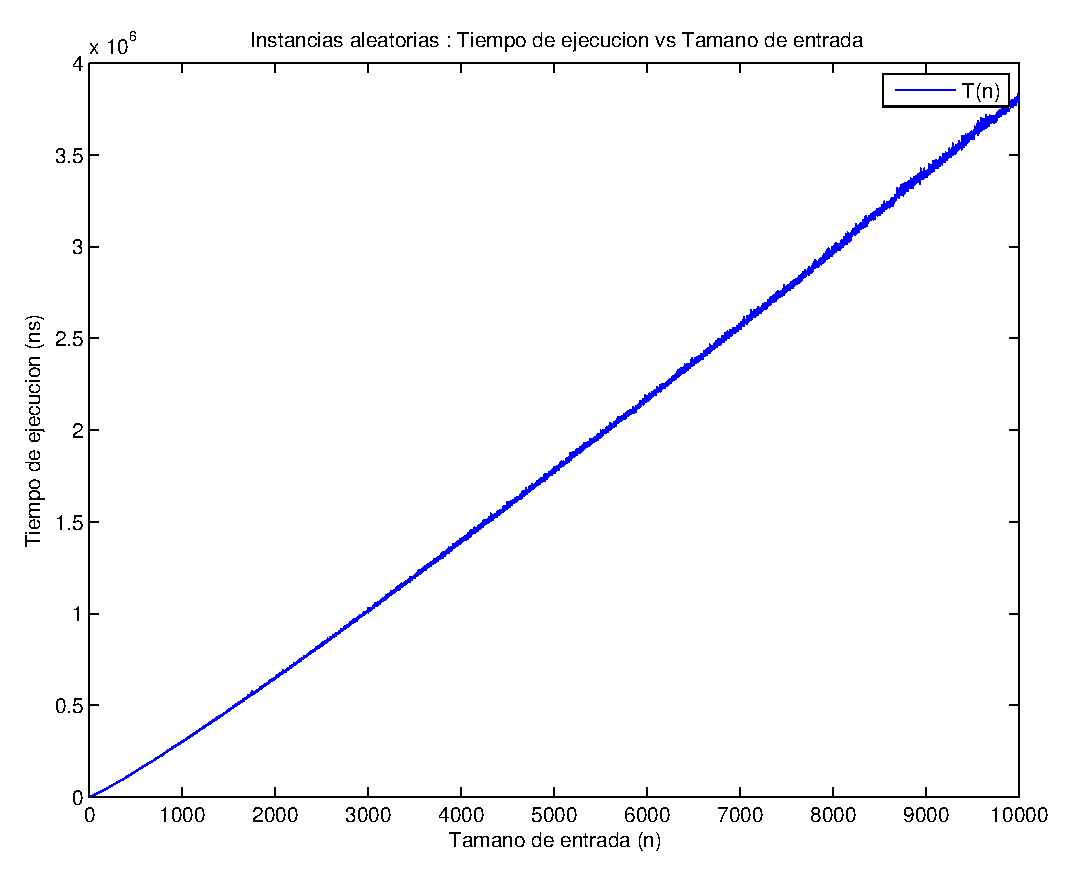
\includegraphics[width=0.5\linewidth]{problema2/graficos/problema2_aleatoria_10000.eps}
    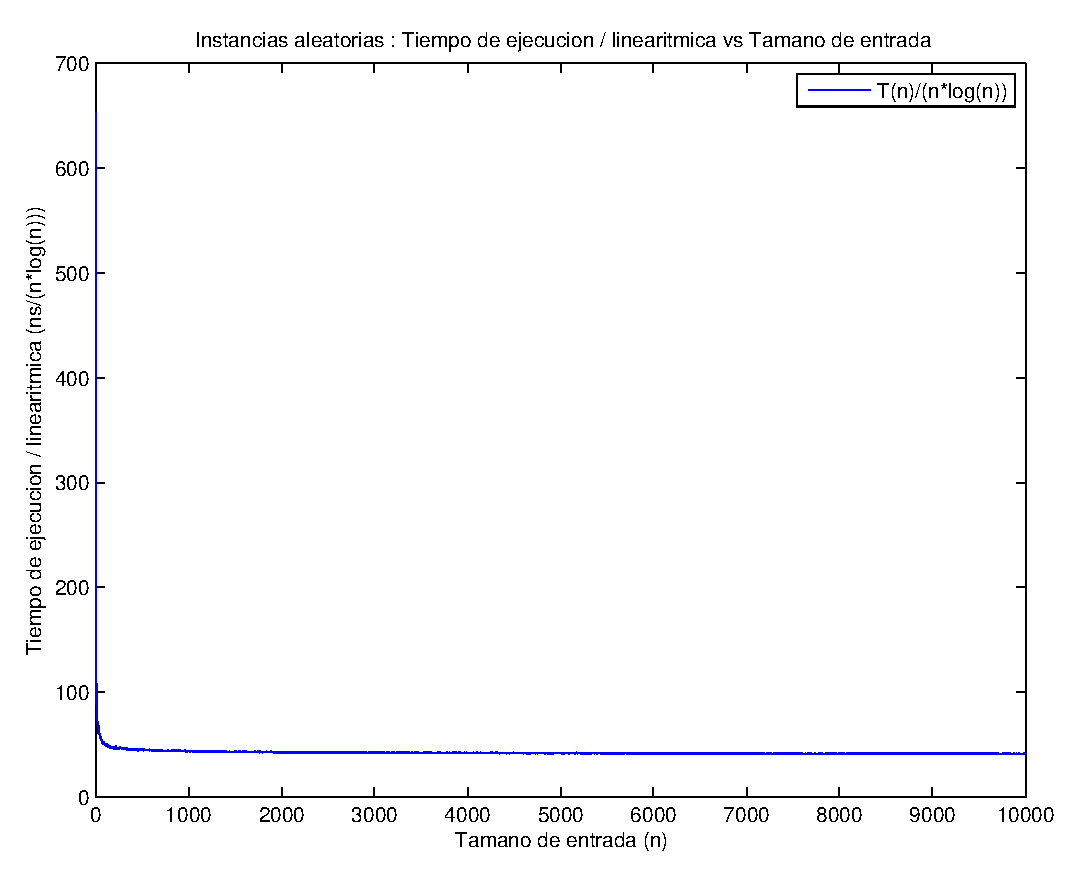
\includegraphics[width=0.5\linewidth]{problema2/graficos/problema2_aleatoria_10000_div_nlogn.eps}
    \caption{Instancias aleatorias, $1 \leq n \leq 10000$. Izquierda: $T(n)$ vs $n$. Derecha: $T(n) / (n * log(n))$ vs $n$.}
    \label{fig:problema2-aleatoria-10000}
  \end{figure}
\end{center}

Además de presentar los datos según fueron medidos, incluímos un gráfico donde se muestra el comportamiento del costo temporal para instancias de tamaño $n$ dividido $n * log(n)$. Esto permite visualizar la tendencia asintótica del cociente $T(n) / (n * log(n))$, que en este caso se aproxima a una constante cercana al valor $50$, sugiriendo dentro del marco de mediciones que $T(n)$ tiende a un crecimiento del orden de $n * log(n)$ para instancias promedio. Esto coincide con el comportamiento observado durante la experimentación del problema \emph{Camiones Sospechosos}, lo cual es de esperarse dado que en ambos casos se utilizó la misma función de ordenamiento para la implementación (ver apéndices \ref{problema1-codigo} y \ref{problema2-codigo}).

Nuevamente, para corroborar que el ciclo posterior al ordenamiento incurre efectivamente en un costo a lo sumo lineal, continuamos la experimentación sobre instancias donde la lista de entrada se encuentra ordenada, eliminando la primer etapa. En este caso, dado que el ciclo no contiene ejecución condicional (siempre ejecuta exactamente la misma cantidad de instrucciones independientemente de la entrada), solo realizamos mediciones sobre instancias pseudo-aleatorias ordenadas según el coeficiente mencionado en \ref{problema2-desarrollo}. En la figura (\ref{fig:problema2-ciclo}) se muestran los resultados.

\begin{center}
  \begin{figure}[H]
    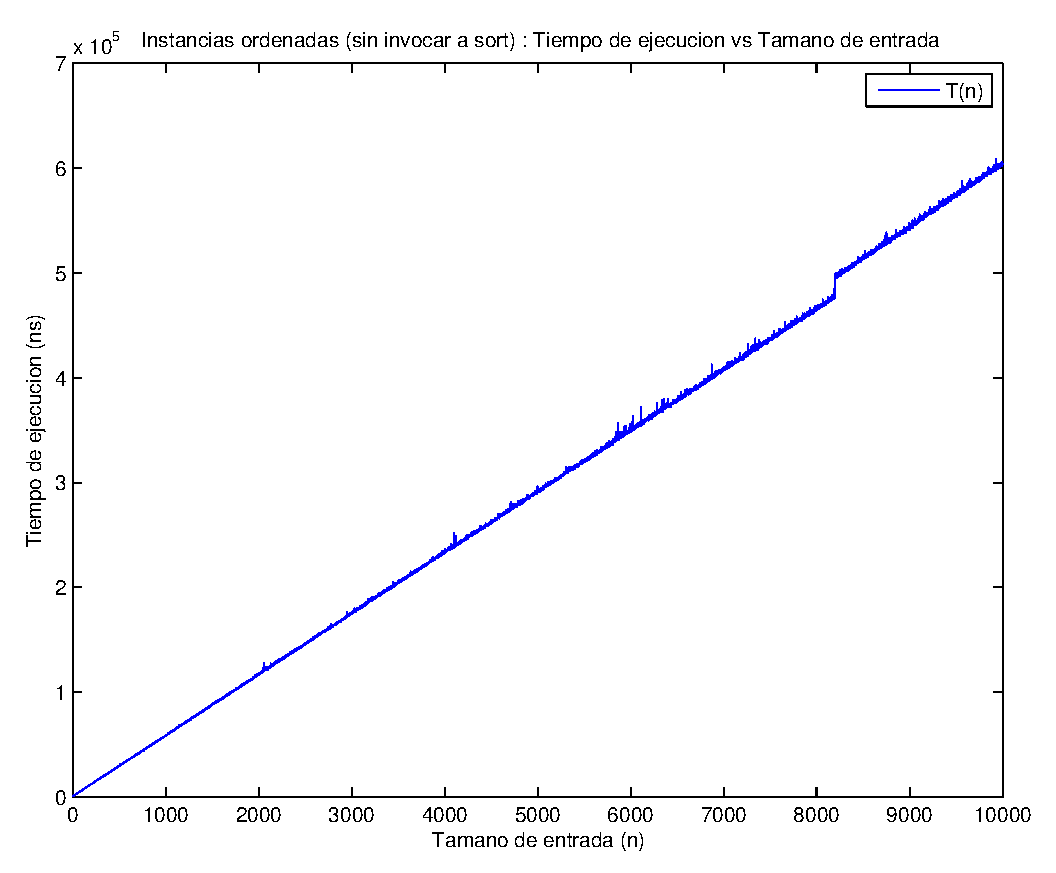
\includegraphics[width=0.5\linewidth]{problema2/graficos/problema2_ordenada_10000.eps}
    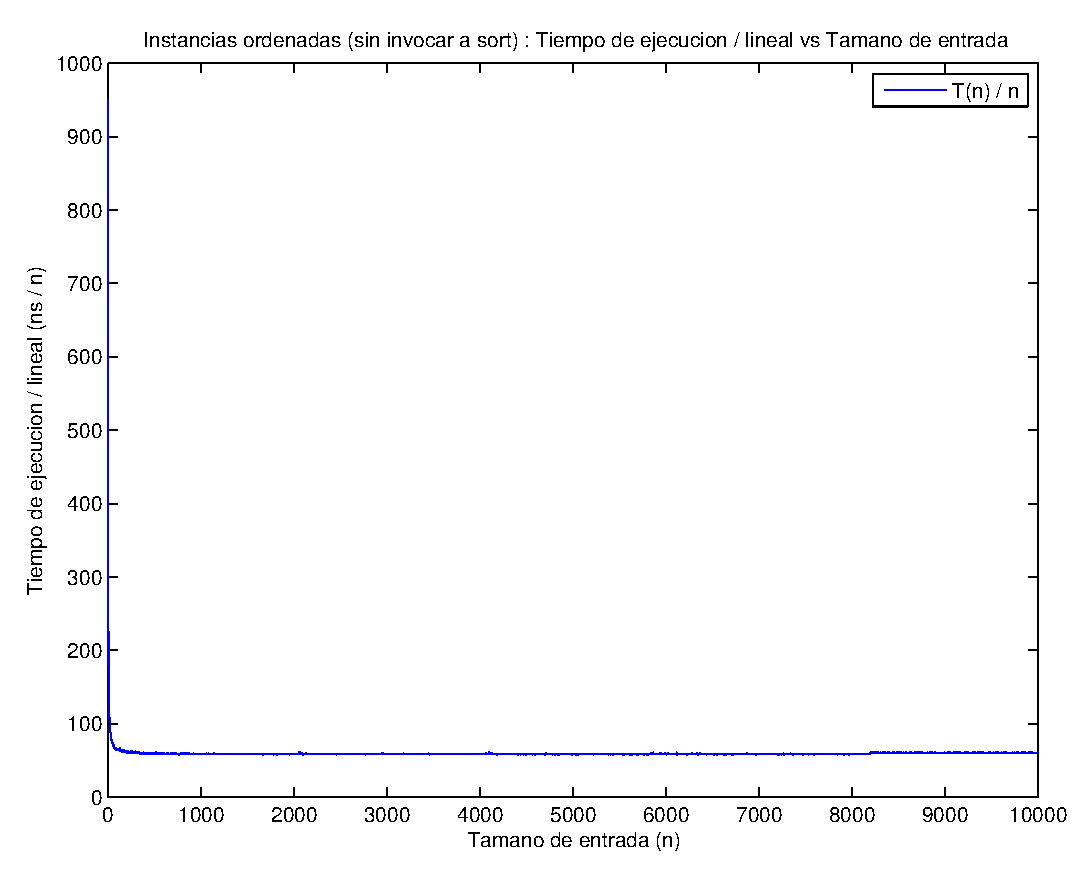
\includegraphics[width=0.5\linewidth]{problema2/graficos/problema2_ordenada_10000_div_n.eps}
  \caption{Instancias aleatorias. $1 \leq n \leq 10000$.}
  \label{fig:problema2-ciclo}
  \end{figure}
\end{center}

Observamos en la curva de costo temporal un crecimiento de orden lineal, con una marcada discontinuidad para $n$ cercano a $8000$. A la vez, incluímos un gráfico mostrando la curva $T(n) / n$ vs $n$\footnote{$T(n)$ en este caso hace referencia a el costo sin la etapa de ordenamiento.}, reiterando sobre la misma técnica utilizada en la sección \ref{problema1-experimentacion}, observando una tendencia hacia un valor constante de aproximadamente $80$ para magnitudes crecientes de $n$. En base a ambas visualizaciones, deducimos que la etapa post-ordenamiento es efectivamente $O(n)$, dado que para la misma no existe distincción entre mejor y peor caso, o caso promedio. Como además es necesario evaluar cada elemento por lo menos una vez al calcular las pérdidas, la etapa es en particular $\Theta(n)$.

Si bien la discontinuidad encontrada no se condice con un comportamiento lineal, aducimos que la misma se debe a cuestiones concretas del contexto de experimentación; por ejemplo, posiblemente debido al tamaño de la memoria caché dado que la posición de la discontinuidad varía cuando realizamos mediciones en equipos de diferentes características.

%Por otro lado, como utilizamos el \emph{sort} de la \emph{stl}, no podemos asegurar si un caso en particular va a ser un ``mejor caso'', o un ``peor caso''. Esto se debe a que, como explicamos anteriormente, el sorting utiliza un \emph{IntroSort} que usa primordialmente un algoritmo similar a \emph{QuickSort}. Por esto al depender del azar, no se puede saber \emph{a priori} si un caso va a ser un ``mejor caso'', o un ``peor caso''.

%Por estas razones, para el ejercicio 2 no incluimos gráficos extra en los cuales hablamos de ``peor caso'' y ``mejor caso''..

\subsection{Resultados y conclusiones}
Dado que el cómputo de la pérdida total tiene un costo fijo determindo por la cantidad de piezas, la variación en el tiempo de ejecución depende exclusivamente del costo de ordenamiento. Por lo tanto, no nos es posible determinar \emph{a priori} si un caso va a resultar mejor o peor para nuestra implementación, sin realizar un complejo análisis de peor caso sobre la función de ordenamiento.

A su vez, la predominancia de la etapa de ordenamiento implica que no va a ser posible mejorar la cota de complejidad teórica de nuestra solución, debido a que los algoritmos de ordenamiento por comparaciones son $\Omega(n * log(n))$.

\newpage


%%%%%%%%%%%%%%%%%%%%%%%%%%%%%%%%%%%%%%%%%%%%%%%%%%%%%%%%%%%%%%%%%%%%%%%%%%%%%%%
%% Apéndices                                                                 %%
%%%%%%%%%%%%%%%%%%%%%%%%%%%%%%%%%%%%%%%%%%%%%%%%%%%%%%%%%%%%%%%%%%%%%%%%%%%%%%%

\begin{appendices}

\section{Código fuente del problema 1}
\label{problema1-codigo}

\verbatiminput{./codigo/problema1.cpp}

\newpage


\section{Código fuente del problema 2}
\label{problema2-codigo}
\verbatiminput{./codigo/problema2.cpp}

\newpage


\section{Código fuente del problema 3}
\label{problema3-codigo}
\verbatiminput{./codigo/problema3.cpp}


\end{appendices}

\end{document}